% !TeX root = ../../../main.tex
\subsubsection{Geometric Constraint Primitives}%
\label{sec:solution.impl.gcps}

Having overcome the language barrier between C++ and Julia, we can build our
\ac{GC} primitives on top of \texttt{CGAL.jl}.  Our implementation follows a
constructive approach where the production of geometry can be done solely
resorting to a straightedge and a compass.  This makes programs easier to
understand and manually reproduce.

The following sections revisit of our initially formulated example problems from
\cref{sec:intro.examples}.

\subsubsection*{Parallel lines}%
\label{sec:solution.impl.gcps.parallel}

Revisiting our earlier examples, we now showcase implementations for those
problems using our solution, accompanied by the Khepri \ac{AD} tool.
\Cref{lst:solution.impl.gcps.parallel} shows a solution to the ``parallel
lines'' problem introduced in \cref{sec:intro.examples.parallel}.

\begin{listing}[htbp]
  \inputminted[highlightlines={4,6-7,16}]{julia}{jl/ex_parallel.jl}
  \caption[Parallel lines example using our solution]{
    Implementation of the parallel lines example illustrated in
    \cref{fig:intro.example.parallel} using Khepri alongside our solution.}%
  \label{lst:solution.impl.gcps.parallel}
\end{listing}

The highlighted \texttt{parallel} function takes a line segment \texttt{l} and a
point \texttt{p} and creates a new line segment starting at point \texttt{p}
with the same length as \texttt{l} , obtained using \texttt{CGAL.jl}'s
\texttt{to\_vector} function.  \Cref{fig:solution.impl.gcps.parallel}
illustrates the program's output in AutoCAD.

\begin{figure}[htbp]
  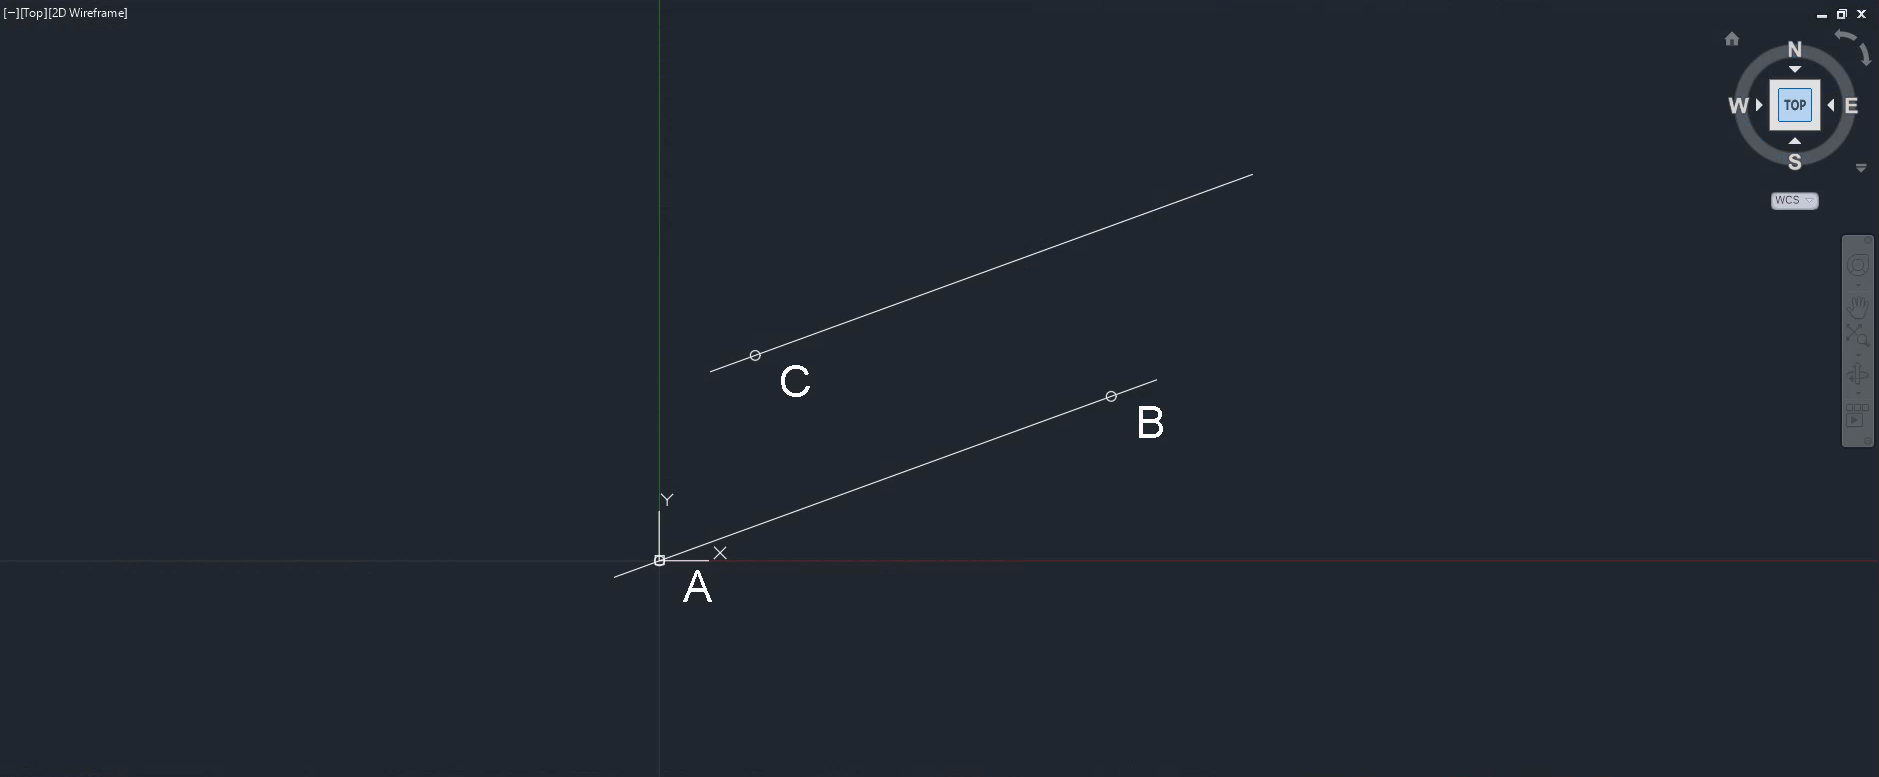
\includegraphics[width=\linewidth]{fig/autocad-parallel} 
  \caption{Parallel lines example using our solution, visualized in AutoCAD\@.}%
  \label{fig:solution.impl.gcps.parallel}
\end{figure}

\subsubsection*{Circumcenter}%
\label{sec:solution.impl.gcps.circumcenter}

We initially solved the circumcenter problem by intersecting triangle sides'
bisectors.  We can still approach the problem that way, defining a
\texttt{circumcenter} function similar to the one in
\cref{lst:solution.impl.gcps.circimpl}.

\begin{listing}[htbp]
  \begin{minted}{julia}
  circumcenter(a, b, c) = intersection(bisector(a, b), bisector(b, c)) 
  \end{minted}
  \caption[Initial circumcenter solution]{
    Initial implementation of \texttt{circumcenter}.}%
  \label{lst:solution.impl.gcps.circimpl}
\end{listing}

However, this functionality is already present in \ac{CGAL}.  This is a perfect
demonstration of our approach's benefits regarding repurposing a comprehensive
library with plenty of functionality.

\Cref{lst:solution.impl.gcps.circumcenter} illustrates a solution to the
``circumcenter'' problem using \ac{CGAL}'s \texttt{circumcenter} function.  The
program's output can be seen in \cref{fig:solution.impl.gcps.circumcenter}.

\begin{listing}[htbp]
  \inputminted[highlightlines={2,4-5,17}]{julia}{jl/ex_circumcenter.jl}
  \caption[Circumcenter example using our solution]{
    Implementation of the circumcenter example illustrated in
    \cref{fig:intro.example.circumcenter} using Khepri alongside our solution.}%
  \label{lst:solution.impl.gcps.circumcenter}
\end{listing}

\begin{figure}[htbp]
  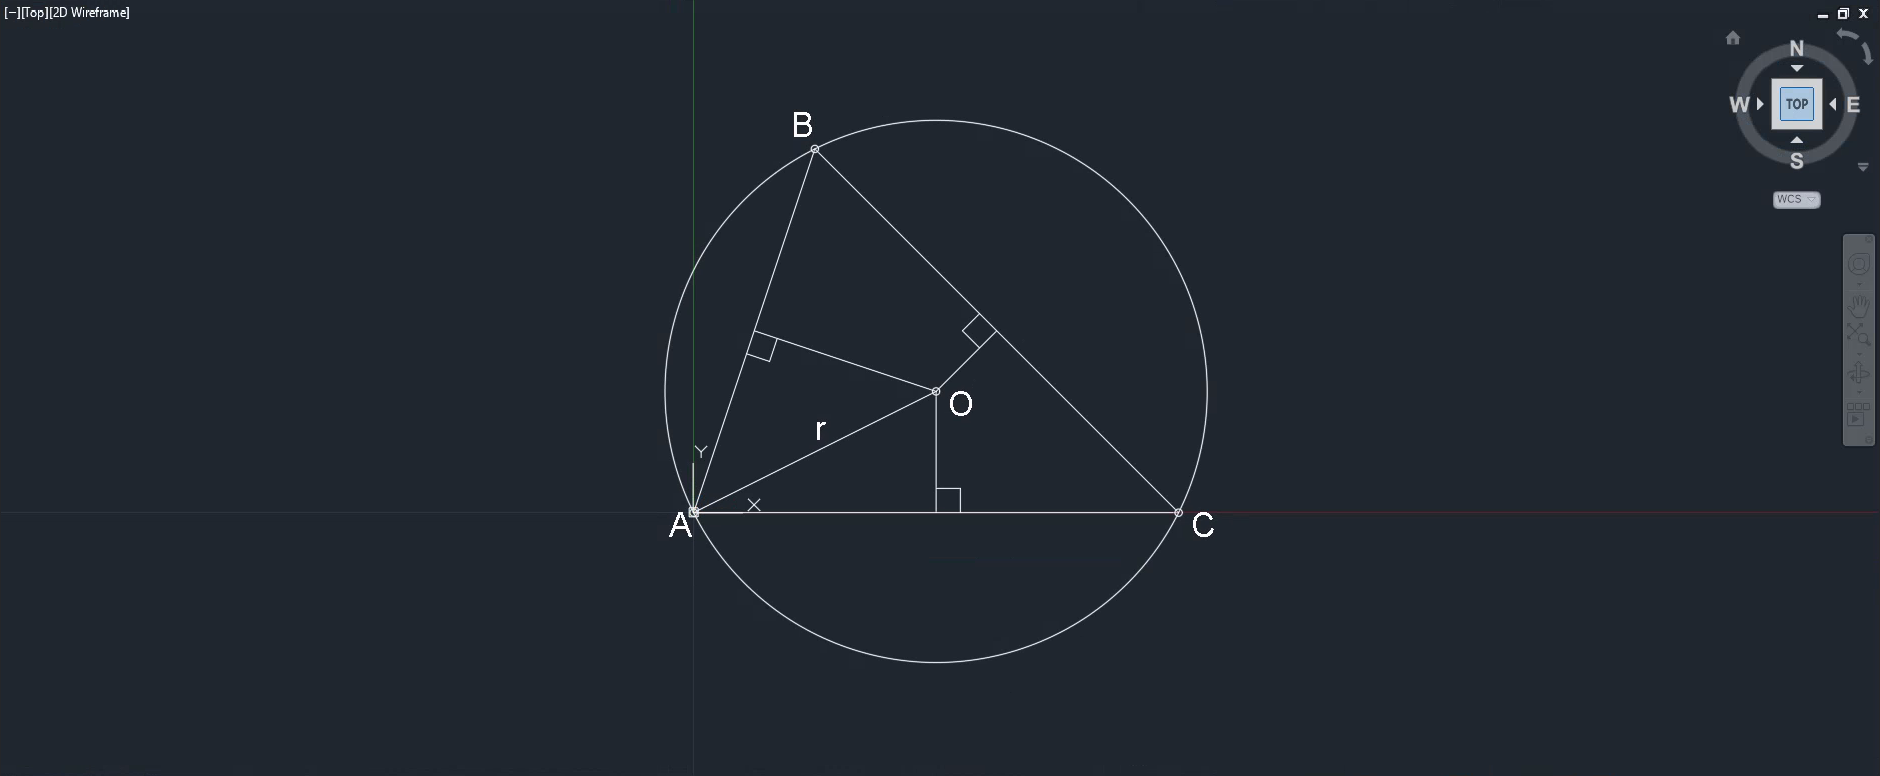
\includegraphics[width=\linewidth]{fig/autocad-circumcenter} 
  \caption[Circumcenter example using our solution]{
    Circumcenter example using our solution, visualized in AutoCAD\@.}%
  \label{fig:solution.impl.gcps.circumcenter}
\end{figure}
